% Math labels
% Made with Xematics. Positions are in px (1 px = 0.75 pt), as in the SVG export.
\documentclass[tikz, border=4pt]{standalone}
\usepackage{amsmath, amssymb}
\definecolor{xm1}{HTML}{FFFFFF}
\definecolor{xm2}{HTML}{D4E8F5}
\definecolor{xm3}{HTML}{0072B2}
\definecolor{xm4}{HTML}{F1F2F4}
\definecolor{xm5}{HTML}{4B5563}
\definecolor{xm6}{HTML}{FBE8C4}
\definecolor{xm7}{HTML}{B97800}
\definecolor{xm8}{HTML}{B8C0CC}
\definecolor{xm9}{HTML}{1F2937}
\definecolor{xm10}{HTML}{6B7280}
\begin{document}
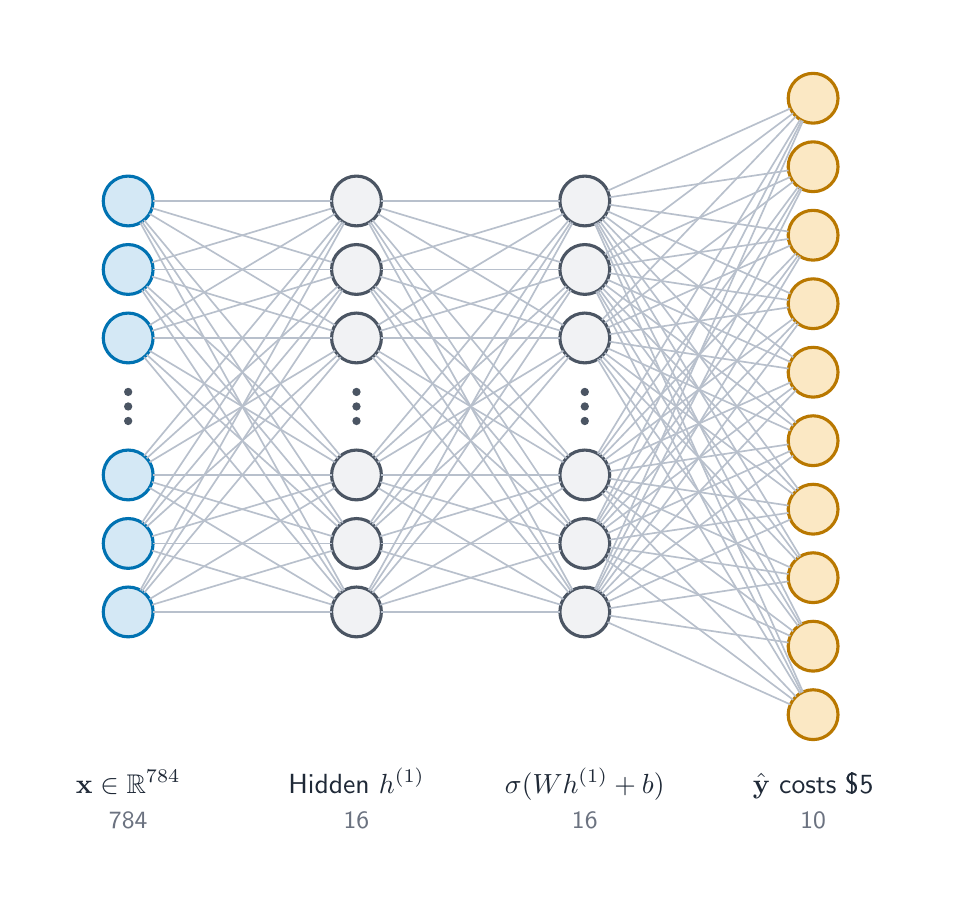
\begin{tikzpicture}[x=0.75pt, y=-0.75pt]
  \tikzset{
    xm input/.style={circle, minimum size=18pt, inner sep=0, outer sep=0, fill=xm2, draw=xm3, line width=1.13pt},
    xm hidden/.style={circle, minimum size=18pt, inner sep=0, outer sep=0, fill=xm4, draw=xm5, line width=1.13pt},
    xm output/.style={circle, minimum size=18pt, inner sep=0, outer sep=0, fill=xm6, draw=xm7, line width=1.13pt},
    xm edge/.style={draw=xm8, line width=0.6pt},
    xm dots/.style={fill=xm5},
    xm name xm9/.style={text=xm9, inner sep=0, font=\sffamily\fontsize{9.75}{11.7}\selectfont},
    xm size xm10/.style={text=xm10, inner sep=0, font=\sffamily\fontsize{9}{10.8}\selectfont},
  }
  \fill[xm1] (0,0) rectangle (433.18,410.82);
  % Neurons
  \node[xm input] (n-0-0) at (48.42,83.5) {};
  \node[xm input] (n-0-1) at (48.42,116.5) {};
  \node[xm input] (n-0-2) at (48.42,149.5) {};
  \node[xm input] (n-0-781) at (48.42,215.5) {};
  \node[xm input] (n-0-782) at (48.42,248.5) {};
  \node[xm input] (n-0-783) at (48.42,281.5) {};
  \node[xm hidden] (n-1-0) at (158.42,83.5) {};
  \node[xm hidden] (n-1-1) at (158.42,116.5) {};
  \node[xm hidden] (n-1-2) at (158.42,149.5) {};
  \node[xm hidden] (n-1-13) at (158.42,215.5) {};
  \node[xm hidden] (n-1-14) at (158.42,248.5) {};
  \node[xm hidden] (n-1-15) at (158.42,281.5) {};
  \node[xm hidden] (n-2-0) at (268.42,83.5) {};
  \node[xm hidden] (n-2-1) at (268.42,116.5) {};
  \node[xm hidden] (n-2-2) at (268.42,149.5) {};
  \node[xm hidden] (n-2-13) at (268.42,215.5) {};
  \node[xm hidden] (n-2-14) at (268.42,248.5) {};
  \node[xm hidden] (n-2-15) at (268.42,281.5) {};
  \node[xm output] (n-3-0) at (378.42,34) {};
  \node[xm output] (n-3-1) at (378.42,67) {};
  \node[xm output] (n-3-2) at (378.42,100) {};
  \node[xm output] (n-3-3) at (378.42,133) {};
  \node[xm output] (n-3-4) at (378.42,166) {};
  \node[xm output] (n-3-5) at (378.42,199) {};
  \node[xm output] (n-3-6) at (378.42,232) {};
  \node[xm output] (n-3-7) at (378.42,265) {};
  \node[xm output] (n-3-8) at (378.42,298) {};
  \node[xm output] (n-3-9) at (378.42,331) {};
  % Connections 0
  \draw[xm edge] (n-0-0) -- (n-1-0);
  \draw[xm edge] (n-0-0) -- (n-1-1);
  \draw[xm edge] (n-0-0) -- (n-1-2);
  \draw[xm edge] (n-0-0) -- (n-1-13);
  \draw[xm edge] (n-0-0) -- (n-1-14);
  \draw[xm edge] (n-0-0) -- (n-1-15);
  \draw[xm edge] (n-0-1) -- (n-1-0);
  \draw[xm edge] (n-0-1) -- (n-1-1);
  \draw[xm edge] (n-0-1) -- (n-1-2);
  \draw[xm edge] (n-0-1) -- (n-1-13);
  \draw[xm edge] (n-0-1) -- (n-1-14);
  \draw[xm edge] (n-0-1) -- (n-1-15);
  \draw[xm edge] (n-0-2) -- (n-1-0);
  \draw[xm edge] (n-0-2) -- (n-1-1);
  \draw[xm edge] (n-0-2) -- (n-1-2);
  \draw[xm edge] (n-0-2) -- (n-1-13);
  \draw[xm edge] (n-0-2) -- (n-1-14);
  \draw[xm edge] (n-0-2) -- (n-1-15);
  \draw[xm edge] (n-0-781) -- (n-1-0);
  \draw[xm edge] (n-0-781) -- (n-1-1);
  \draw[xm edge] (n-0-781) -- (n-1-2);
  \draw[xm edge] (n-0-781) -- (n-1-13);
  \draw[xm edge] (n-0-781) -- (n-1-14);
  \draw[xm edge] (n-0-781) -- (n-1-15);
  \draw[xm edge] (n-0-782) -- (n-1-0);
  \draw[xm edge] (n-0-782) -- (n-1-1);
  \draw[xm edge] (n-0-782) -- (n-1-2);
  \draw[xm edge] (n-0-782) -- (n-1-13);
  \draw[xm edge] (n-0-782) -- (n-1-14);
  \draw[xm edge] (n-0-782) -- (n-1-15);
  \draw[xm edge] (n-0-783) -- (n-1-0);
  \draw[xm edge] (n-0-783) -- (n-1-1);
  \draw[xm edge] (n-0-783) -- (n-1-2);
  \draw[xm edge] (n-0-783) -- (n-1-13);
  \draw[xm edge] (n-0-783) -- (n-1-14);
  \draw[xm edge] (n-0-783) -- (n-1-15);
  % Connections 1
  \draw[xm edge] (n-1-0) -- (n-2-0);
  \draw[xm edge] (n-1-0) -- (n-2-1);
  \draw[xm edge] (n-1-0) -- (n-2-2);
  \draw[xm edge] (n-1-0) -- (n-2-13);
  \draw[xm edge] (n-1-0) -- (n-2-14);
  \draw[xm edge] (n-1-0) -- (n-2-15);
  \draw[xm edge] (n-1-1) -- (n-2-0);
  \draw[xm edge] (n-1-1) -- (n-2-1);
  \draw[xm edge] (n-1-1) -- (n-2-2);
  \draw[xm edge] (n-1-1) -- (n-2-13);
  \draw[xm edge] (n-1-1) -- (n-2-14);
  \draw[xm edge] (n-1-1) -- (n-2-15);
  \draw[xm edge] (n-1-2) -- (n-2-0);
  \draw[xm edge] (n-1-2) -- (n-2-1);
  \draw[xm edge] (n-1-2) -- (n-2-2);
  \draw[xm edge] (n-1-2) -- (n-2-13);
  \draw[xm edge] (n-1-2) -- (n-2-14);
  \draw[xm edge] (n-1-2) -- (n-2-15);
  \draw[xm edge] (n-1-13) -- (n-2-0);
  \draw[xm edge] (n-1-13) -- (n-2-1);
  \draw[xm edge] (n-1-13) -- (n-2-2);
  \draw[xm edge] (n-1-13) -- (n-2-13);
  \draw[xm edge] (n-1-13) -- (n-2-14);
  \draw[xm edge] (n-1-13) -- (n-2-15);
  \draw[xm edge] (n-1-14) -- (n-2-0);
  \draw[xm edge] (n-1-14) -- (n-2-1);
  \draw[xm edge] (n-1-14) -- (n-2-2);
  \draw[xm edge] (n-1-14) -- (n-2-13);
  \draw[xm edge] (n-1-14) -- (n-2-14);
  \draw[xm edge] (n-1-14) -- (n-2-15);
  \draw[xm edge] (n-1-15) -- (n-2-0);
  \draw[xm edge] (n-1-15) -- (n-2-1);
  \draw[xm edge] (n-1-15) -- (n-2-2);
  \draw[xm edge] (n-1-15) -- (n-2-13);
  \draw[xm edge] (n-1-15) -- (n-2-14);
  \draw[xm edge] (n-1-15) -- (n-2-15);
  % Connections 2
  \draw[xm edge] (n-2-0) -- (n-3-0);
  \draw[xm edge] (n-2-0) -- (n-3-1);
  \draw[xm edge] (n-2-0) -- (n-3-2);
  \draw[xm edge] (n-2-0) -- (n-3-3);
  \draw[xm edge] (n-2-0) -- (n-3-4);
  \draw[xm edge] (n-2-0) -- (n-3-5);
  \draw[xm edge] (n-2-0) -- (n-3-6);
  \draw[xm edge] (n-2-0) -- (n-3-7);
  \draw[xm edge] (n-2-0) -- (n-3-8);
  \draw[xm edge] (n-2-0) -- (n-3-9);
  \draw[xm edge] (n-2-1) -- (n-3-0);
  \draw[xm edge] (n-2-1) -- (n-3-1);
  \draw[xm edge] (n-2-1) -- (n-3-2);
  \draw[xm edge] (n-2-1) -- (n-3-3);
  \draw[xm edge] (n-2-1) -- (n-3-4);
  \draw[xm edge] (n-2-1) -- (n-3-5);
  \draw[xm edge] (n-2-1) -- (n-3-6);
  \draw[xm edge] (n-2-1) -- (n-3-7);
  \draw[xm edge] (n-2-1) -- (n-3-8);
  \draw[xm edge] (n-2-1) -- (n-3-9);
  \draw[xm edge] (n-2-2) -- (n-3-0);
  \draw[xm edge] (n-2-2) -- (n-3-1);
  \draw[xm edge] (n-2-2) -- (n-3-2);
  \draw[xm edge] (n-2-2) -- (n-3-3);
  \draw[xm edge] (n-2-2) -- (n-3-4);
  \draw[xm edge] (n-2-2) -- (n-3-5);
  \draw[xm edge] (n-2-2) -- (n-3-6);
  \draw[xm edge] (n-2-2) -- (n-3-7);
  \draw[xm edge] (n-2-2) -- (n-3-8);
  \draw[xm edge] (n-2-2) -- (n-3-9);
  \draw[xm edge] (n-2-13) -- (n-3-0);
  \draw[xm edge] (n-2-13) -- (n-3-1);
  \draw[xm edge] (n-2-13) -- (n-3-2);
  \draw[xm edge] (n-2-13) -- (n-3-3);
  \draw[xm edge] (n-2-13) -- (n-3-4);
  \draw[xm edge] (n-2-13) -- (n-3-5);
  \draw[xm edge] (n-2-13) -- (n-3-6);
  \draw[xm edge] (n-2-13) -- (n-3-7);
  \draw[xm edge] (n-2-13) -- (n-3-8);
  \draw[xm edge] (n-2-13) -- (n-3-9);
  \draw[xm edge] (n-2-14) -- (n-3-0);
  \draw[xm edge] (n-2-14) -- (n-3-1);
  \draw[xm edge] (n-2-14) -- (n-3-2);
  \draw[xm edge] (n-2-14) -- (n-3-3);
  \draw[xm edge] (n-2-14) -- (n-3-4);
  \draw[xm edge] (n-2-14) -- (n-3-5);
  \draw[xm edge] (n-2-14) -- (n-3-6);
  \draw[xm edge] (n-2-14) -- (n-3-7);
  \draw[xm edge] (n-2-14) -- (n-3-8);
  \draw[xm edge] (n-2-14) -- (n-3-9);
  \draw[xm edge] (n-2-15) -- (n-3-0);
  \draw[xm edge] (n-2-15) -- (n-3-1);
  \draw[xm edge] (n-2-15) -- (n-3-2);
  \draw[xm edge] (n-2-15) -- (n-3-3);
  \draw[xm edge] (n-2-15) -- (n-3-4);
  \draw[xm edge] (n-2-15) -- (n-3-5);
  \draw[xm edge] (n-2-15) -- (n-3-6);
  \draw[xm edge] (n-2-15) -- (n-3-7);
  \draw[xm edge] (n-2-15) -- (n-3-8);
  \draw[xm edge] (n-2-15) -- (n-3-9);
  % Layers
  \fill[xm dots] (48.42,175.5) circle[radius=2];
  \fill[xm dots] (48.42,182.5) circle[radius=2];
  \fill[xm dots] (48.42,189.5) circle[radius=2];
  \fill[xm dots] (158.42,175.5) circle[radius=2];
  \fill[xm dots] (158.42,182.5) circle[radius=2];
  \fill[xm dots] (158.42,189.5) circle[radius=2];
  \fill[xm dots] (268.42,175.5) circle[radius=2];
  \fill[xm dots] (268.42,182.5) circle[radius=2];
  \fill[xm dots] (268.42,189.5) circle[radius=2];
  % Labels
  \node[xm name xm9, anchor=base] at (48.42,368.75) {$\mathbf{x} \in \mathbb{R}^{784}$};
  \node[xm size xm10, anchor=base] at (48.42,385.93) {784};
  \node[xm name xm9, anchor=base] at (158.42,368.75) {Hidden $h^{(1)}$};
  \node[xm size xm10, anchor=base] at (158.42,385.93) {16};
  \node[xm name xm9, anchor=base] at (268.42,368.75) {$\sigma(W h^{(1)} + b)$};
  \node[xm size xm10, anchor=base] at (268.42,385.93) {16};
  \node[xm name xm9, anchor=base] at (378.42,368.75) {$\hat{\mathbf{y}}$ costs \$5};
  \node[xm size xm10, anchor=base] at (378.42,385.93) {10};
\end{tikzpicture}
\end{document}
